\documentclass[11pt]{article}
\usepackage[top=1.00in, bottom=1.0in, left=1in, right=1in]{geometry}
\renewcommand{\baselinestretch}{1.1}
\usepackage{Sweave}
\usepackage{graphicx}
\usepackage{natbib}
\usepackage{amsmath}
\usepackage{gensymb}
\usepackage{parskip}
\usepackage{xcolor}
\usepackage{xr-hyper}
\externaldocument{bayesianflows}

\def\labelitemi{--}

\usepackage{fancyhdr}
\pagestyle{fancy}
\fancyhead[LO]{}
\fancyhead[RO]{}

\begin{document}
\bibliographystyle{/Users/Lizzie/Documents/EndnoteRelated/Bibtex/styles/besjournals}

\renewcommand{\refname}{\CHead{}}

\title{Supplement: A four-step Bayesian workflow for improving ecological science}
\date{\today}
\author{EM Wolkovich, TJ Davies, WD Pearse \& M Betancourt}
\maketitle

\renewcommand{\thetable}{S\arabic{table}}
\renewcommand{\thefigure}{S\arabic{figure}}

\section*{A brief review of statistical inference using Bayesian approaches}

Robust analyses ely on our inferences being consistent with the underlying truth more often than not.  Quantifying this consistency is calibration---analyzing how often a parameter estimate is close to the true value---a critical part of using models for inference. A major problem with traditional (frequentist) approaches in ecology today is their inferences are unpredictable when their foundational assumptions are not met, but ecologists are not usually trained in how to recognize or deal with this.
% Most ecologists are trained primarily in frequentist methods, which are focused on calibration (this is is why training in frequentist methods includes so much discussion of significance, power, mean squared error, and the like). Bayesian methods typically focus on inference, but can be equally well calibrated (see Step 1, below). 

To better understand our workflow, we provide a very brief overview of some of the fundamentals of Bayesian methods that is inherently incomplete and, by design, not very technical. This section can be skipped for those who feel already well-versed, and can be augmented for those who are new to Bayesian approaches \citep[for example,][]{statrethink,BDA,regotherstories}.

Probability is often defined as ``the long-term frequency with which something happens.'' We would expect, for example that if we tossed a coin 100 times we would see roughly 50 heads.  In this case we would say that the probability of tossing a coin and getting a `head' is $\frac{50}{100}$, equivalent to 50\% or $\frac{1}{2}$. At the same time we wouldn't be very surprised if we observed 49 or even 55 heads, although we would be surprised if we saw 99.

This definition of probability---which is the \emph{frequentist} definition---is useful in many situations, but it has a few disadvantages. First, frequentist definitions aren't very helpful when dealing with unexpected situations. Frequentist probabilities are grounded in repeatable observations, and so understanding these repeatable frequencies is of limited use when trying to make predictions for changing or entirely novel systems. Second, most common frequentist approaches rely on specific assumptions. Using frequentist statistics requires trying to match a model that we have (often just in our heads) of some ecological system to a frequentist method that mostly closely matches the assumptions of our biological model. Given the complexity of ecological data and our uncertainty about the underlying model, frequentist approaches can be especially challenging in ecology. 

Bayesian approaches provide a way to build models that can propagate our (un)certainties about what we do---or especially, don't---know about how ecological systems work. In the Bayesian view, $probability$ is used to quantify uncertainty: the higher the probability of a certain interval of values the less uncertainty we have that the true behavior falls within that interval. Assuming we also have some estimate of our initial uncertainty---usually from knowledge of ecology---to inform a prior distribution (termed below $prior$), then we can apply Bayes' theorem:

\begin{equation}
  probability = \frac{likelihood \cdot prior}{normaliser}
  \label{bayes_theorem}
\end{equation}

to update that prior into a posterior distribution that accounts for the information added by a likelihood ($likelihood$ is the same as a frequentist likelihood). Here, \texttt{normaliser} is a mathematical constant that makes sure our probability cannot go above 100\% or below 0\% (statisticians are lazy, and will not `give 110\%'). This mathematical constant [technically it is the probability of our data; $p(data)$] is a nuisance term that is extremely challenging to estimate (sometimes it is impossible!) and held back the practical use of Bayesian statistics for almost a century because that normaliser could rarely be analytically worked out. But one of the major advantages of Bayesian methods is that the solution to this problem---numerical simulations based on Markov Chain Monte Carlo (MCMC)---provide a huge additional advantage. Now that no analytical solution needs be found, any model that can be written out mathematically can be fit to data, giving the scientist more freedom of model structure.

% Nowadays, with increases in computer power, we can use numerical methods such as `Markov Chain Monte Carlo' (MCMC) methods to avoid having to estimate its value precisely. Such methods are iterative algorithms  that involve chance at each step (that the process proceeds in iterations or steps, and only the last iteration affects the next, is why this is a `Markov Chain'), tweaking and changing parameters within your model until a distribution of parameters consistent with the data are found. This distribution is called the `posterior' distribution to distinguish how it is our view of probability \emph{after} the data (via the likelihood) and the prior have been considered. %There is no guarantee that the posterior distribution will, itself, be found: the user must check for so-called `convergence' onto the true posterior distribution as the process involves randomness. It is for this randomness that `Monte Carlo' is added into the name, after a city famous for gambling.

% It turns out there is a further advantage that such an approach gives us. While frequentist probabilities are all about the probabilities of observing data ($p(data|model)$: what are the chances of getting 99 heads in 100 coin-tosses?), Bayesian probabilities are all about the probabilities of observing models ($p(model|data)$: what are the chances this coin is biased towards heads?). This makes it straightforward to report the results of Bayesian analyses in terms of estimates of uncertainty and precision of coefficients (contrast ``I'm 80\% certain that coin comes up heads at least two-thirds of the time'' with ``I'm less than 5\% certain those last twenty coin tosses came from a fair coin'').

\section*{Which workflow?}

Formally, all a `workflow' does is organize various steps together in a systematic fashion, but there are many different workflows depending on what the aim is, which will determine which steps a workflow should include. For example a workflow aimed at calibration could look like an expanded version of our Step 1, where all the steps focus on investigating the assumptions encoded in a given model using simulated data. Or a workflow aimed at inference could expand Step 3, to focus on constructing a posterior, then investigating its model adequacy via several criteria. An inferential workflow can also be extended into a model development workflow.  If the model adequacy criteria inform not only that something is inadequate about the current model assumptions but what is inadequate (ideally this happens some in Step 4) then one can use those hints to iterative improve the modeling assumptions. We present in the main text a very simplified model development workflow that combines calibration, inference and some model development, but it is not necessarily appropriate for everyone, depending on their aims.

% Ultimately it may be helpful to advocate for workflows, plural.  Bayesian methodologies can be used to systematically investigate the consequences of a given model, such as an estimator calibration workflow.  They can also be used to formalize heuristic residual checking with posterior retrodictive check and implement an iterative model development workflow.  Etc, etc.  The goal is to identify what you want to do and organize the steps to achieve that output as systematically as possible.


\section*{An example workflow}

Our workflow is explained mostly program-agnostically. Though at times we assume a user of \textsf{Stan}, a relatively new probabalistic programming language, that interfaces with \textsf{R, Python, Julia} (and more) to write bespoke Bayesian models \citep{Carpenter:2017stan}. We focus on \textsf{Stan} as its MCMC algorithm (a variant of Hamiltonian Monte Carlo, HMC) is fast and produces specific output to warn of model fit issues (i.e., divergent transitions) in a way other MCMC algorithms do not (e.g. Metropolis-Hastings or Gibbs), but the basic workflow should apply to diverse implementations of Bayesian modeling, and can be extended to other approaches (frequentist, resampling, etc.). \\ % to write bespoke Bayesian models and underpins the \textsf{R} packages \textsf{brms} and \textsf{rstanarm}, which fit a suite of specific (pre-defined) models

% From Mike: To adjust and add this general caveat:
one of the common problems, especially for people who are used to building analyses from black box components, is that transitioning to more flexible techniques is often overwhelming.  Even if the ideas are compelling the open-endedness in the implementation can discourage people who experiment, causing them to default back to the status quo.

The benefit of a longer presentation with comprehensive examples is that the reader directly sees how all of these conceptual pieces fall into a practical implementation and how straightforward that implementation can be in the context of a particular application.  Generalizing to bespoke applications will still be frustrating, but at least they're walking in the right direction.


We review our workflow using an example from the first Bayesian model one of us ever fit. The resulting model is not ideal (as we'll show), but we use it to highlight the reality of the learning the skills of this workflow. Much like learning a foreign language you improve over time, to where you almost cannot fathom where you started. And when you're first learning a foreign language the stories you can tell will be crude and  clunky, but as you become more proficient they'll become more elaborate.

Our example comes from a project aiming to estimate levels of trophic (a)synchrony with climate change. Using observational time-series data, we wanted to estimate changes in the relative timing of species pairs. We had data on Acartia hudsonica unique species from 1951 to 2013  and thought we should fit a mixed-model linear regression, with day of year (calendar day, so 1-366) of event as the response and year as the predictor. Given variable time-series length we thought we should set species as a `random effect' of species on the intercept and slope and so tried:

\begin{Schunk}
\begin{Sinput}
> modelwanted <- lmer(phenovalue~(year|species), data=d) 
\end{Sinput}
\end{Schunk}

but that did not work; the model returned: \textt{boundary (singular) fit: see help('isSingular')}. We could get the same model with a `random effect' of species on the intercept only and that's what we would often have put in a paper. In the language of the day, we had `controlled' for non-independence in our data and so could have reported this model:

\begin{Schunk}
\begin{Sinput}
> modelconverged <- lmer(phenovalue~year+(1|species), data=d)
\end{Sinput}
\end{Schunk}

But we knew this was not right: our understanding of climate change impacts suggested it was highly unlikely all species have a common change over time. So we tried a Bayesian approach to ideally fit separate slopes for each species over time, but drawn from a common distribution (which is what the term `random effect' generally refers to in ecology) and started thinking about our model. 

Even before we arrived at the data simulation step, we realized our verbal model did not agree with the statistical model we expected to fit. We planned to fit a simple linear model, but that would assume climate change has been ongoing across all our years and that's not what most science on anthropogenic warming suggests: it suggests instead a large uptick in warming around 1980 \citep[likely do to effects of aerosols,][]{Booth2012}. So instead we developed a `hinge' model to fit the linear regression after 1980 and a mean before 1980. This highlights a reality throughout the workflow: effective model building is about efficient brainstorming. It's a constant back and forth between asking questions about what we know and what we should know. 

\emph{Step 1:}
 
Next we simulated data to test our model code. To do this we set the parameters as our first step, then we simulate the data  from these set parameters. In simulation, we know the `truth'---which here is a our model parameters---and we then compare those with what we estimated to what we started with.
 
\begin{Schunk}
\begin{Sinput}
>  # Create the species-level parameters
> Nspp <- 50
> mu_doy <- 125
> sigma_doy <- 20
> mu_shift <- 0.5
> sigma_shift <- 5
> species_doy <- rnorm(Nspp, mu_doy, sigma_doy)
> species_trend <- rnorm(Nspp, mu_shift, sigma_shift)
> # Create the overall `error'
> sigma_y <- 5
> # Create the data
> year_0 <- 1980
> n_data_per_species <- round(runif(Nspp, 5, 40))
> species <- rep(1:Nspp, n_data_per_species)
> N <- length(species)
> year <- rep(NA, N)
> for (sp in 1:Nspp){
+   year[species==sp] <- rev(2009 - 1:(n_data_per_species[sp])) - year_0
+ }
> ypred <- length(N)
> for (n in 1:N){
+   s <- species[n]
+   ypred[n] <- species_doy[s] + species_trend[s]*year[n]
+ }
> y <- rnorm(N, ypred, sigma_y)
\end{Sinput}
\end{Schunk}

 And checked that it returned our results:
 
 ....


These sorts of simulation studies are  exactly how power is formally defined. Thus, these simulations allow us to estimate power in more general conditions that what is typically assumed for analytic results.

\emph{Step 2}

\emph{Step 3}

\emph{Step 4}

At this step, we actually realized the partial pooling on our intercept was not a good fit to the data (Fig. \ref{fig:ppmodels}). We assumed from the beginning that we should partially pool on the intercepts because that is how fixing `non-independence' with `random effects' is taught in ecology, but our retrodictive checks made us think twice. We realized that we had data from diverse events across locations and their average values were unlikely to be normally distributed (though they may be if we had focused on a certain more local area, such as temperate sites in Europe. We ended up with partial pooling only on the slopes and not intercepts---a model that made biological sense, but we never would have considered without this workflow. 


\section{References}
\vspace{-5ex}
\bibliography{refs/bayesrefsmini.bib}

\clearpage
\section{Figures}

\begin{figure}[ht]
\centering
\noindent 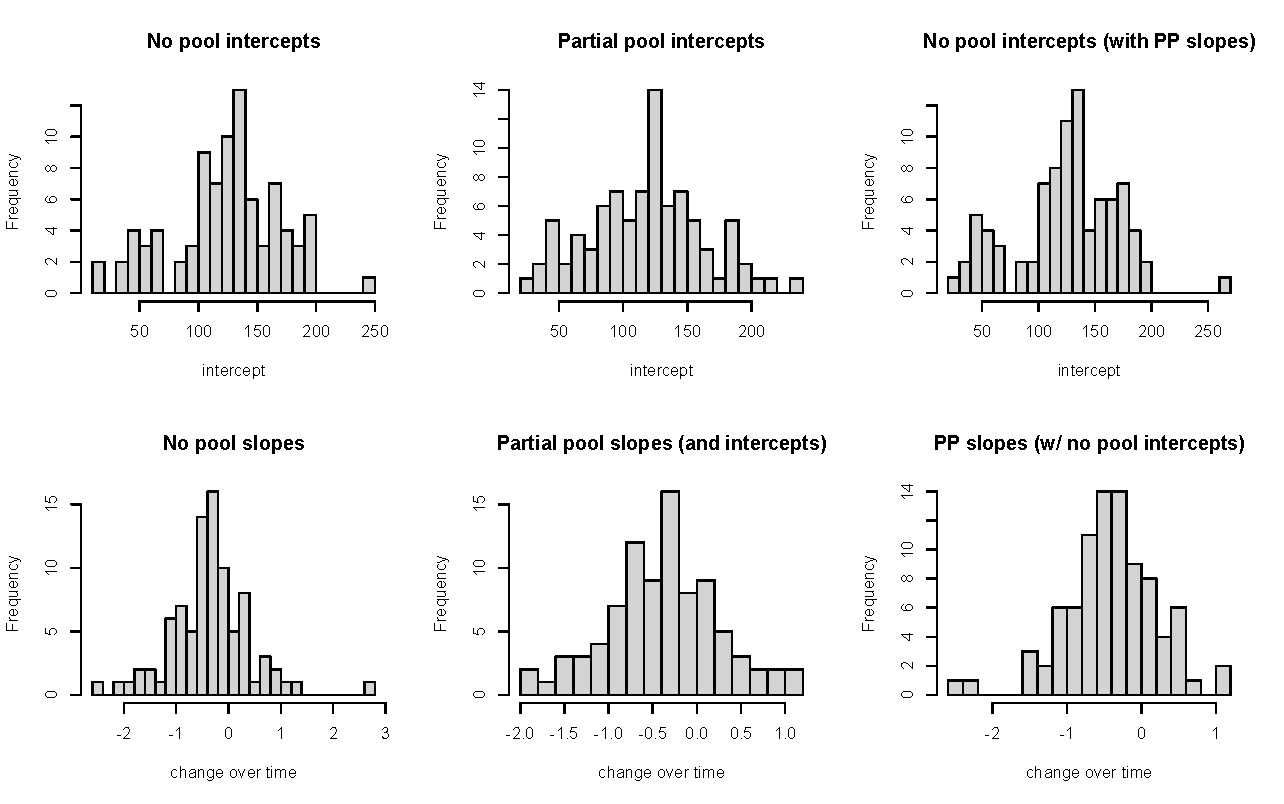
\includegraphics[width=1\textwidth]{examples/synchrony/graphs/compareppmodels.pdf}
\caption{Comparison of three types of models we fit: no pooling (right), partial pooling on slopes and intercept (middle) and partial pooling on slopes only (left).}
\label{fig:ppmodels}
\end{figure}

\end{document}


\section{Where to next?}

% Our workflow and its description is brisk, and thus anyone wanting to implement it would benefit from more reading. There are new good resources on this sort of workflow, and more being published often, but for now we especially recommend: 

Our workflow and its description is brisk, and thus anyone wanting to implement it would benefit from more reading. We highlight some good resources on this sort of workflow in the main text. More are being published often, so we recommend checking for new resources, but here's a smattering of things to check out currently:

Mike's workflow

Any good vingettes?

Aki's course on ROS?

\cite{esfahani2021bayesian,schad2021,schad2022workflow}


I think that it would also be useful to mention residual analysis. Overall we need to compare model retrodictions to the observed data, projected onto the features relevant to the analysis. Classical residual analysis compares point predictions to the observe data. R2 summarizes this comparison as a linear correlation. Posterior retrodictive checks compare an entire distribution of predictions to the observed data, allowing us to not only identify any inconsistencies but also use the probabilistic spread of the predictions to qualify how important any inconsistencies are.

Feedbacks 

`Developing simulated data to test the model, running prior and retrodictive checks all dive you deep into understanding
your statistical model, which suddenly you may find yourself thinking through much more mechanistically.' I wonder if
it's beneficial to frame this more as `dive deep into connecting your statistical model to your domain expertise'?  I
often find myself trying to emphasize that people already have the domain expertise but they're not incorporating it into
their analyses.  A lot of what this workflow is trying to do is facilitate that integration to leverage what the analysts
have always had!
